\lstset{
	language=[Visual]C++,
	keywordstyle=\bfseries\sffamily\color[rgb]{0,0,1},
	identifierstyle=\sffamily,
	commentstyle=\color[rgb]{0.133,0.545,0.133},
	stringstyle=\sffamily\color[rgb]{0.627,0.126,0.941},
	showstringspaces=false,
	basicstyle=\small,
	numberstyle=\footnotesize,
	numbers=left,
	stepnumber=1,
	numbersep=10pt,
	tabsize=2,
	breaklines=true,
	prebreak = \raisebox{0ex}[0ex][0ex]{\ensuremath{\hookleftarrow}},
	breakatwhitespace=false,
	aboveskip={1.5\baselineskip},
	columns=fixed,
	upquote=true,
	extendedchars=true,
}

\section{Auto Triggering Function Generator\label{cp:AutoTriggeringFunctionGenerator}}
Some applications require internal periodic or random triggering. The \deviceName\ function generator provides this functionality.\par

The delay between two trigger pulses of this trigger generator is the sum of two components: A fixed value M and a pseudo random value given by the exponent N. \par

The period is

\begin{align}
    T = 1 + M + [1...2^N]
\end{align}

clock cycles \ifxHPTDC{of the 150~MHz clock}{with a duration of $4~ns$ per cycle}.\par

The trigger can be used as a source for the TiGer unit (see Section \ref{cp:tiger}).


\section{Timing Generator (TiGer)\label{cp:tiger}}
Each digital LEMO-00 input can be used as a \ifxHPTDC{AC coupled}{LVCMOS} trigger output. 
The TiGer function can be configured independently for each connector. 
See Section \ref{cp:tigerblock} for a full description of the configuration options.
% 
\begin{figure*}[ht]
    \begin{center}
        \ifxHPTDC { 
            % this is an XCIrcuit drawing  convertex from postscript with 
            %ps2pdf.exe -dEPSCrop xhptdc8_trigger_matrix.ps
            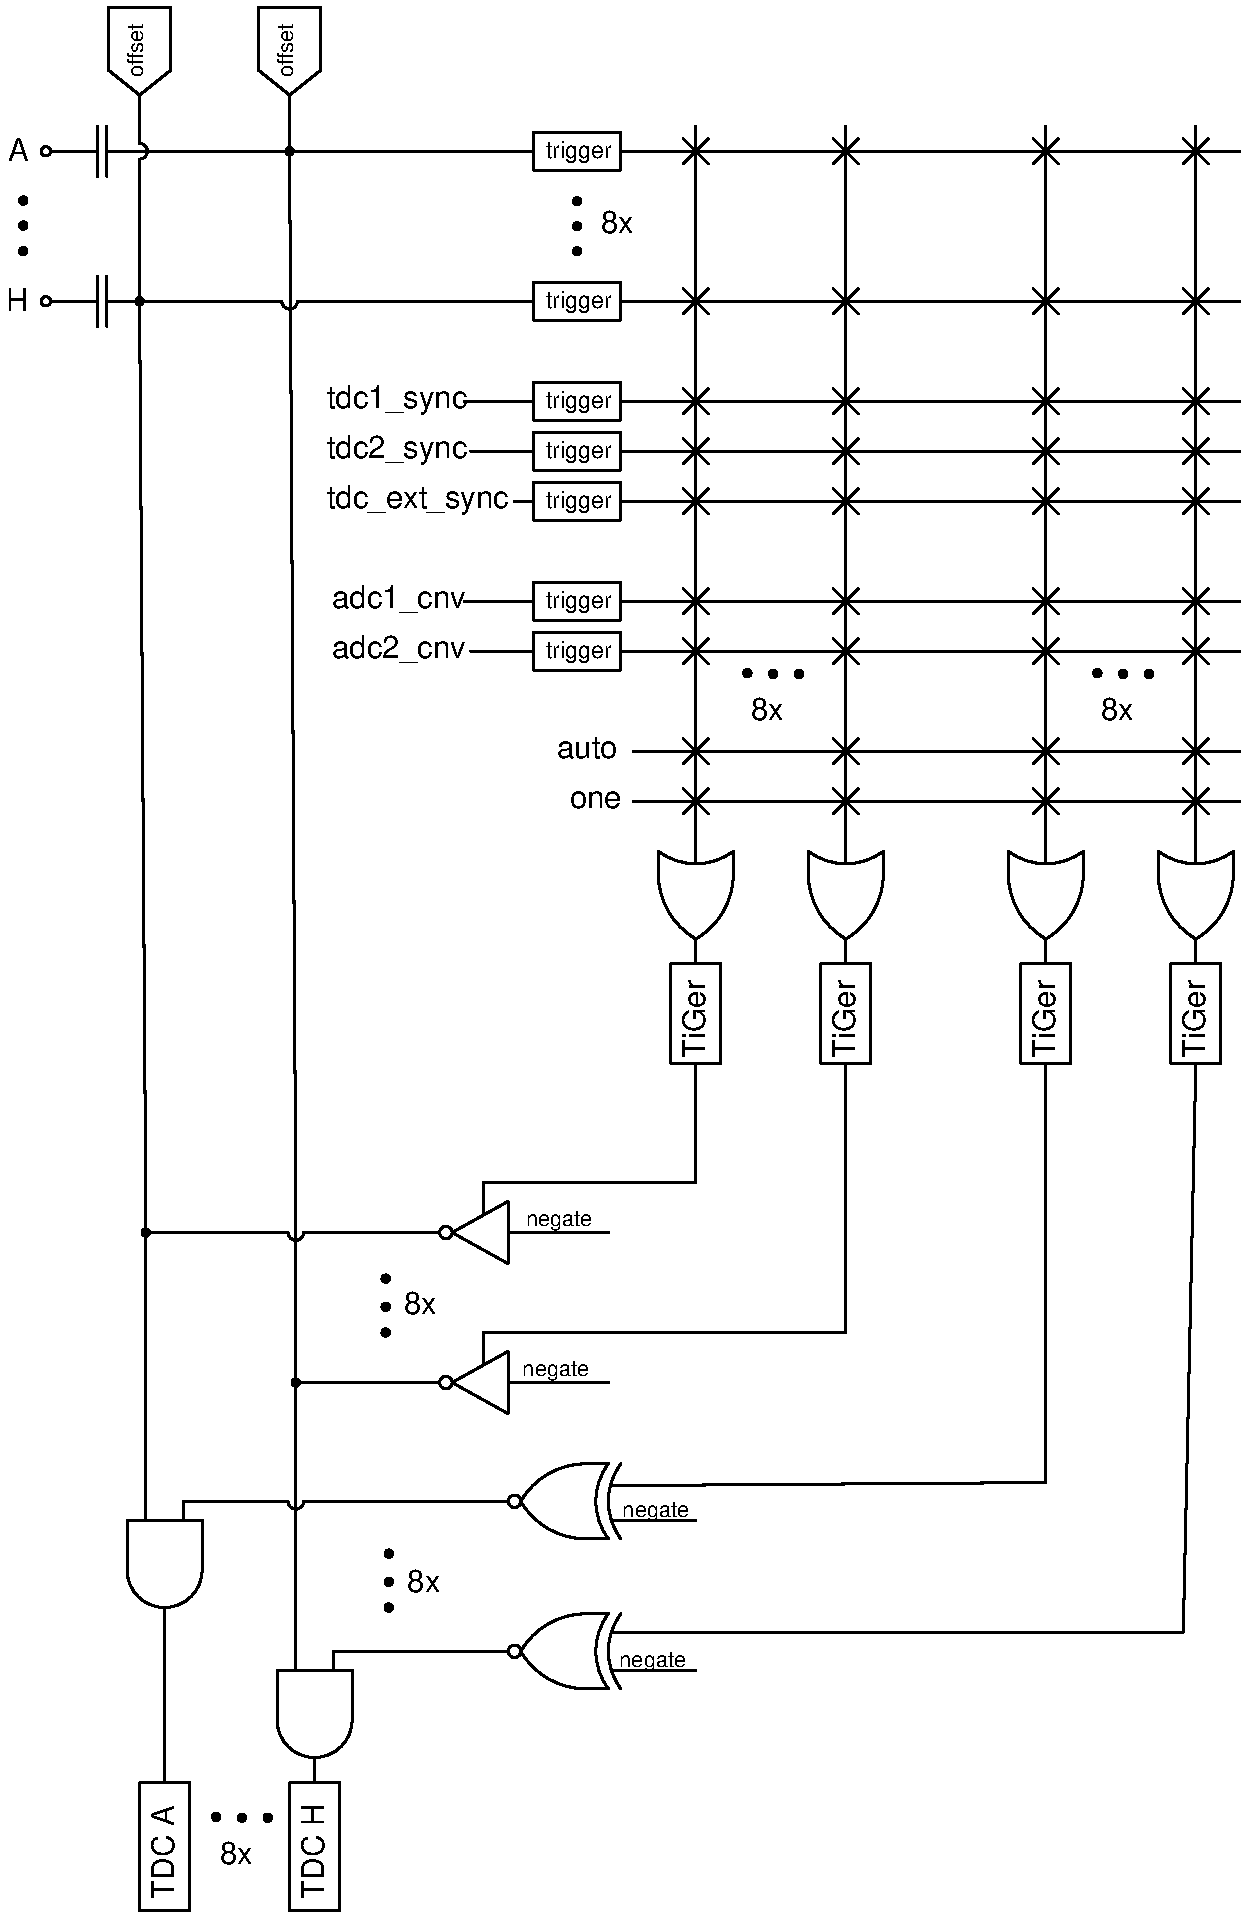
\includegraphics[width=0.6\textwidth]{xhptdc/figures/xhptdc8_trigger_matrix.pdf}
        }{
            \includegraphics[width=0.7\textwidth]{figures/xTDC4_tiger_matrix.pdf}
        }
        \caption{TiGer blocks can generate outputs that are also available on inputs.\label{fig:matrix}} 
    \end{center}
\end{figure*}
%

Figure \ref{fig:matrix} shows how the TiGer blocks are connected. They can be triggered by an OR of an arbitrary combination of inputs, 
including the auto trigger. Each TiGer can drive its output to its corresponding LEMO connector. This turns the connector into an output. 

When there is an ADC trigger pulse on the TRG connector, either of the two on board ADCs is triggered in an unpredictable pattern. 
If the TRG input shall be used as a trigger the trigger sources must be contain both \textsf{ADC1\tu CNV} and \textsf{ADC21\tu CNV}.

The trigger sources with names ending in \textsf{\tu sync} are managed by the driver for multi board setups and must be left unchanged by the user.

\ifxHPTDC{
	The TiGer outputs are AC coupled to the connector. They can be operated in one of the following modes:
	\paragraph*{\textsf{\PREFIX\tu TIGER\tu OFF}} 
		No signal is output to the connetor. 
	\paragraph*{\textsf{\PREFIX\tu TIGER\tu OUTPUT}} 
		In this mode the connector is input only. Pulses are unipolar with 2V amplitude. 
		Connected hardware must not drive any signals to connectors used as outputs, as doing so could damage both the \deviceName and the external hardware. 
		We recommend to only use short pulses to avoid undesirable baseline shift due to the AC coupling, but the device does not pose any restrictions on the duty cycle. 
		This mode can be used as a clock output with a frequency of $75/N$~MHz for integer $N$.
	\paragraph*{\textsf{\PREFIX\tu TIGER\tu BIDI}} 
		In this mode the TiGer creates unipolar pulses with 1~V amplitude. The connector can still be used as an input. 
		Use short pulses to keep the propability of collision and the effect on the baseline low.	
	\paragraph*{\textsf{\PREFIX\tu TIGER\tu BIPOLAR}} 
		In this mode the connector creates bipolar pulses with 1~V amplitude. The connector can still be used as an input. 
		The pulses have no effect on the baseline offset. 
		TiGer should be configured with $stop = start$ for minimum width bipolar pulses of $2 \times 6.\overline{6}~ns$. 
		The maximum bipolar pulse width is \textsf{XHPTDC8\tu TIGER\tu MAX\tu BIPOLAR\tu PULSE\tu LENGTH = 15}.    
}{
	The TiGer is DC coupled to the connector. Connected hardware must not drive any signals to connectors used as outputs, 
	as doing so could damage both the \deviceName\  and the external hardware.
	Pulses that are short enough for the input AC coupling are available as input signals to the \deviceName. 
	This can be used to measure exact time differences between the generated output signals and input signals on other channels.
}
\ttinput{Tiger_Example.tex}	

\ifxHPTDC{
	\subsection{Triggering the ADC with the TiGer}
		\label{adctiger}
		There is a ninth TiGer that is connected to the trigger input of the ADC. See section \ref{adc} for additional information on the ADC. 

		The ADC TiGer can be used with retrigger enabled to periodically sample ADC data. 
		The period should be no shorter than 300~ns or 45 TiGer clocks.

		The ADC TiGer can also be used to sample voltages at a time relative to one of the TDC inputs. In this case 
		stop should be set to at least 45 to ensure that the sample period criterion is met even when pulses
		arrive in quick succession. A typical application would be to sample some slow control voltage once per start signal.

	\section{Gating}
		Each TDC channel has a second TiGer block that functions as a gate as shown in figure \ref{fig:matrix}. 
		While that output of that gating block is active no hits are recorded in that channel.
		If the block is negated hits are only recorded while the gating block is active.
		
		This is a useful feature in setups where the trigger creates a lot of noise.
		A suitable configuration of the gating block can reduce the bandwidth and buffer usage significantly.
		Gating is performed before the L0 buffer. Grouping is performed in software after readout. 
		
	\section{Triggerable ADC}
		\label{adc}
		The \deviceName\ is equipped with a triggerable ADC. 
		Whenever there is a rising edge on the ADC trigger connector, 
		the voltage on the ADC input connector is sampled. 
		The result is inserted as a packet with timestamp and ADC value into the readout data stream.

		The ADC trigger also is connected to the output of a TiGer block. 
		This can be used to to trigger the ADC periodical or relative to one of the TDC input as described in section \ref{adctiger}

		The ADC triggers should not be closer than 300ns apart.

		There are two interleaved ADCs  to ensure that there is always an ADC available even during readout. 
		This is exposed to the user both in the output data format and in the TiGer and Gating trigger sources.
		When using the ADC trigger as a trigger for Gating or TiGer both trigger sources shall be set to the same value.
		During readout the user shall not distinguish between data from the two ADCs unless advanced calibration is 
		desired for the ADC data. In that case the two ADCs should be treated separately.   

}{}